\chapter{Desenvolvimento}

Parte principal do trabalho, que contém a exposição ordenada e pormenorizada do assunto. É composta de revisão de literatura, dividida em seções e subseções, material e métodos e/ou metodologia e resultados, agora descritos detalhadamente. Cada seção ou subseção deverá ter um título apropriado ao conteúdo.

Deve-se utilizar sempre a terceira pessoa do singular na elaboração do texto, mantendo-se a forma impessoal.

\section{Regras gerais de apresentação}

Constituem-se como padrão para apresentação de trabalhos acadêmicos:

\begin{itemize}
\item Tamanho da fonte: Arial ou Times New Roman, tamanho 12. Deve-se utilizar apenas um dos tipos escolhidos em todo o trabalho. Fonte tamanho 10 para citações de mais de três linhas, notas de rodapé e legendas, corpo e fonte das ilustrações e tabelas e paginação.
\item Formato do título: o título do trabalho, na capa e na folha de rosto, deve aparecer em CAIXA ALTA, negrito, centralizado e fonte tamanho 12. Havendo subtítulo, este deve ser precedido por dois pontos, escrito também em CAIXA ALTA, negrito e sem ponto final;
\item Parágrafo: com recuo na primeira linha de 1,5 cm., justificado, sem espaçamento anterior ou posterior.
\end{itemize}

\section{Margens}
Utilizar margens esquerda e superior de 3 cm; e margens direita e inferior de 2 cm; Tamanho do papel: A4; Cabeçalho e rodapé: 1,25 cm.

\section{Espaçamento}

As notas, as referências e a natureza do trabalho devem ser digitadas em espaço simples; Todo o texto deve ser formatado com espaço de 1,5 cm entre linhas (sem espaçamento antes/depois).

As citações com mais de três linhas (longas) são em espaço simples e com recuo de 4 cm da margem esquerda. ``As referências devem ser elaboradas em espaço simples, alinhadas à margem esquerda do texto e separadas entre si por uma linha em branco de espaço simples''~\cite{NBR6023:2018}.

\section{Ilustrações}

São ilustrações: f\textbf{iguras, quadros, gráficos, fotografias}, retratos, desenhos, gravuras, imagens, fluxogramas, organogramas, esquemas, mapas, plantas e \textbf{diferenciam-se das tabelas}. As ilustrações devem ser inseridas o mais próximo possível do texto a que se refere, mas mantendo um espaço (1,5 cm) de separação.

Qualquer que seja o tipo de ilustração, sua identificação deve ser posicionada na parte \textbf{superior}, precedida da palavra designativa, seguida de seu número de ordem de ocorrência no texto, em algarismos arábicos, do respectivo título e/ou legenda. A fonte deve ser tamanho 10. Após a legenda, deve-se apresentar ilustração e em seguida citar a fonte de onde foi retirada a ilustração, exemplo: Fonte: Autor (data), bem comodeve-se referenciá-la, de forma completa, na seção Referências. 

* Para inserir legendas nas ilustrações e tabelas: 

\begin{enumerate}
    \item Na guia \textbf{Referências}, no grupo \textbf{Legendas}, clicar em \textbf{Inserir Legenda}.
    \item Na lista \textbf{Rótulo}, selecionar o rótulo que descreve melhor o objeto. Se a lista não contiver o rótulo correto, clicar em \textbf{Novo Rótulo}, digitar o novo rótulo na caixa \textbf{Rótulo} e clicar em \textbf{OK}.
    \item Digitar o texto, incluindo a pontuação que deseja exibir depois do rótulo e clicar \textbf{enter} para utilizar a formatação apropriada para a Fonte.
\end{enumerate}

\textcolor{red}{Utilizar sempre a primeira linha da folha, em todo o trabalho. A seguir, um modelo de formatação de figura:}

\newpage



\begin{figure}[!htb]%% Ambiente figure
     %\captionsetup{width=0.55\textwidth}%% Largura da legenda
     \caption{As dimensões curriculares de pré-escolar}%% Legenda
     \label{fig:exemplo2}%% Rótulo
     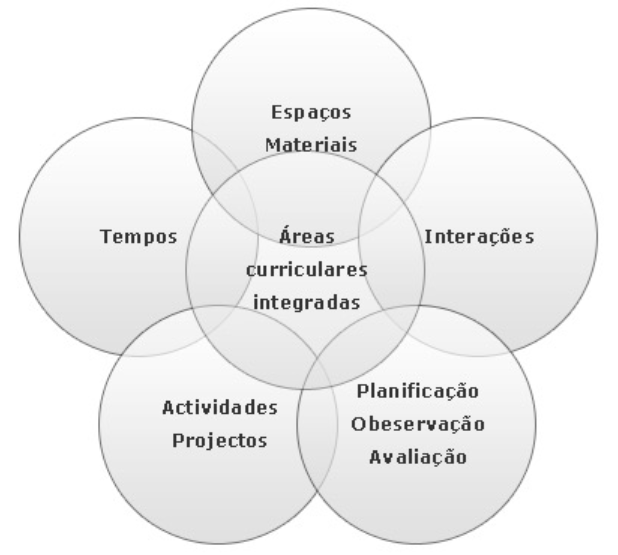
\includegraphics[scale=0.5]{FigDimCurriculares}%% Dimensões e localização
     \fonte{\citeonline{Centro:2025}}%% Fonte
     \addcontentsline{loge}{figure}{\protect\numberline{\thefigure}As dimensões curriculares de pré-escolar}
 \end{figure}

Texto, texto, texto, texto, texto, texto, texto, texto, texto, texto, texto, texto.


\begin{figure}[!htb]%% Ambiente figure
     %\captionsetup{width=0.55\textwidth}%% Largura da legenda
     \caption{Glândulas exócrinas e endócrinas}%% Legenda
     \label{fig:exemplo3}%% Rótulo
     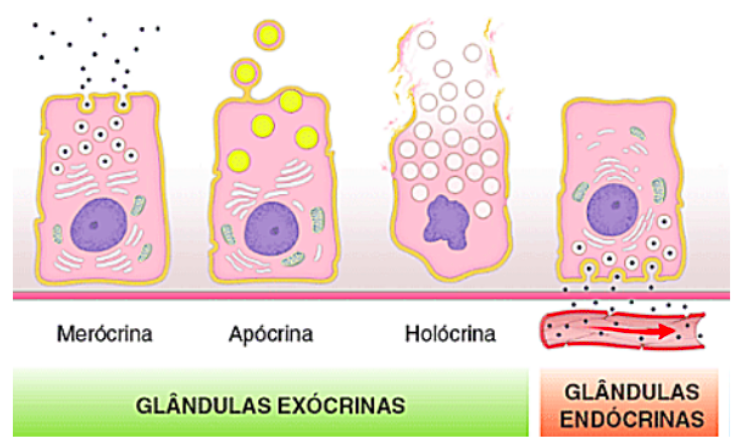
\includegraphics[scale=0.5]{glandulas}%% Dimensões e localização
     \fonte{Adaptado de \citeonline[p.~144]{Pawlina:2018}}%% Fonte
     \addcontentsline{loge}{figure}{\protect\numberline{\thefigure}Glândulas exócrinas e endócrinas}
 \end{figure}


\noindent\textcolor{red}{A seguir, um modelo de formatação de fotografia:}

\newpage

 \begin{photograph}[!htb]%% Ambiente figure
      %\captionsetup{width=0.55\textwidth}%% Largura da legenda
      \caption{Entrada do antigo Departamento de Biblioteca da UTFPR Campus Ponta Grossa}%% Legenda
      \label{fig:foto1}%% Rótulo
      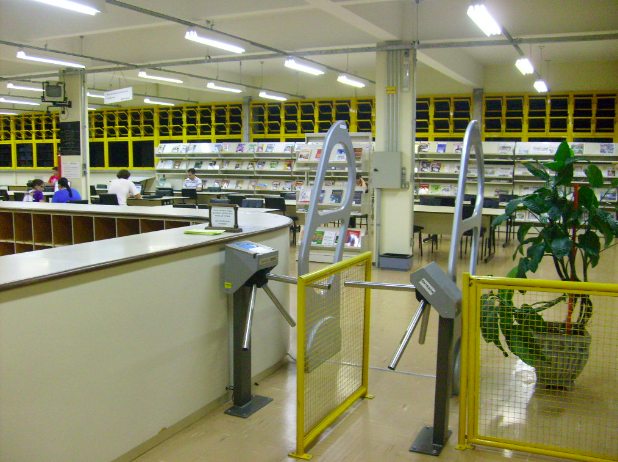
\includegraphics[scale=0.5]{fotografia1}%% Dimensões e localização
      \fonte{Autoria própria (2014)}%% Fonte
      \addcontentsline{loge}{photograph}{\protect\numberline{\thephotograph}Entrada do antigo Departamento de Biblioteca da UTFPR Campus Ponta Grossa} % Adiciona à lista de ilustrações
  \end{photograph}

\noindent\textcolor{red}{\textbf{Atenção:} As fontes das ilustrações e tabelas também deverão constar na lista de referências, ou indicar como Fonte: Autoria própria (ano), se for o caso. Na UTFPR adotou-se negrito e centralizado nas legendas e fonte das ilustrações e tabelas.}

 \begin{photograph}[!htb]%% Ambiente figure
      %\captionsetup{width=0.55\textwidth}%% Largura da legenda
      \centering
      \caption{Entrada da Biblioteca Mario Vargas Llosa, Lima (Peru), também conhecida como ``Casa de la Literatura Peruana''. Em destaque, o primeiro tipógrafo adquirido na América Latina}%% Legenda
      \label{fig:foto2}%% Rótulo
      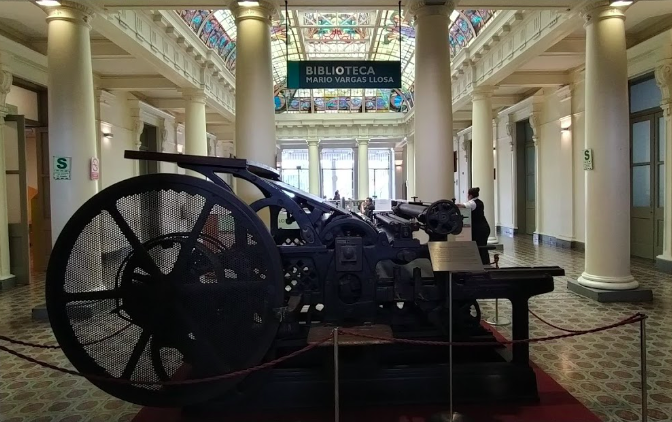
\includegraphics[scale=0.5]{fotografia2}%% Dimensões e localização
      \fonte{Autoria própria (2019)}%% Fonte
      \addcontentsline{loge}{photograph}{\protect\numberline{\thephotograph}Entrada da Biblioteca Mario Vargas Llosa, Lima (Peru), também conhecida como ``Casa de la Literatura Peruana''. Em destaque, o primeiro tipógrafo adquirido na América Latina} % Adiciona à lista de ilustrações
  \end{photograph}

 \textcolor{red}{A seguir, um modelo de formatação de gráfico:}

 \newpage

 \begin{graph}[!htb]%% Ambiente figure
      %\captionsetup{width=0.55\textwidth}%% Largura da legenda
      \caption{Estatística de empréstimos domiciliares realizados em janeiro de 2019 pelas Bibliotecas da UTFPR}%% Legenda
      \label{fig:grap1}%% Rótulo
      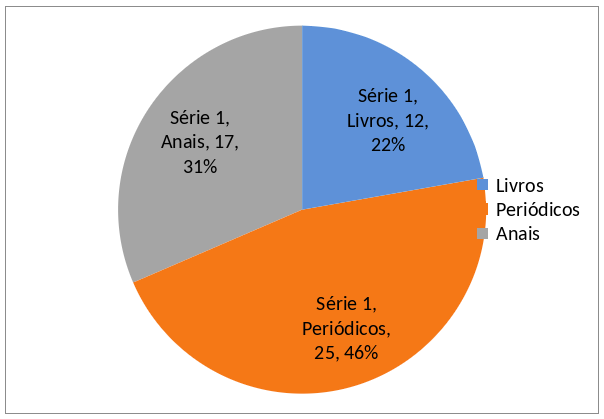
\includegraphics[scale=0.5]{grafico1a}%% Dimensões e localização
      \fonte{\citeonline{UTFPR2020}}%% Fonte
      \addcontentsline{loge}{graph}{\protect\numberline{\thephotograph}Estatística de empréstimos domiciliares realizados em janeiro de 2019 pelas Bibliotecas da UTFPR} % Adiciona à lista de ilustrações
  \end{graph}

Texto, texto, texto, texto, texto, texto, texto, texto, texto, texto, texto, texto, texto, texto, texto, texto, texto, texto, texto, texto, texto, texto, texto, texto, texto.

\textcolor{red}{Modelo de formatação de quadros (prevalecem informações textuais).}

\begin{tabframed}[htb]%% Ambiente tabframed
 %\captionsetup{width=0.5\textwidth}%% Largura da legenda
 \caption{Áreas de desenvolvimento de competências na organizações (pública e privada)}%% Legenda
 \label{quad:exemplo1}%% Rótulo
 \renewcommand{\arraystretch}{1.5}
 \begin{tabular}{|l|p{9cm}|}
 \cline{1-2}
 \multicolumn{1}{|c|}{\textbf{Áreas de desenvolvimento}} & \multicolumn{1}{|c|}{\textbf{\centering Descrição}}\\ \cline{1-2}
  1. Competências sobre processos & Conhecimento nos processos de trabalho \\ \cline{1-2}  
  2. Competências técnicas & Conhecimento técnico nas tarefas a serem desempenhadas e tecnologias empregadas nestas tarefas \\ \cline{1-2}  
  3. Competências sobre a organização & Saber organizar os fluxos de trabalho \\ \cline{1-2}
  4. Competências de serviço & Aliar as competências técnicas com o impacto que estas ações terão para o cliente consumidor \\ \cline{1-2}
  5. Competências sociais & Atitudes que sustentam o comportamento do indivíduo: saber comunicar-se e responsabilizar-se pelos seus atos.\\ \cline{1-2}
 \end{tabular}
 \fonte{\citeonline{FLEURY:2018}}%% Fonte
 \addcontentsline{loge}{tabframed}{\protect\numberline{\thetabframed}Áreas de desenvolvimento de competências na organizações (pública e privada)}
 \end{tabframed}

\textcolor{red}{Para quadros que ocupam mais de uma folha, não é necessária nenhuma sinalização (continua/continuação/conclusão). Apenas nas tabelas se faz necessária essa sinalização}

Texto, texto, texto, texto, texto, texto, texto, texto, texto, texto, texto, texto.

\newpage

\section{Tabelas}

Deve-se seguir tal padrão em todo o trabalho, constando também na lista de tabelas, separada da lista de ilustrações. \textcolor{red}{As tabelas se diferenciam dos quadros por não apresentarem os fechamentos laterais.}\footnote{Para as regras gerais de apresentação das tabelas consultar: IBGE (Instituto Brasileiro de Geografia e Estatística). \textbf{Normas para Apresentação Tabular}. 3. ed. Rio de Janeiro: IBGE, 1993. Disponível em: http://biblioteca.ibge.gov.br/visualizacao/livros/liv23907.pdf
}

\vspace{1cm}

\textcolor{red}{Modelo de formatação de tabelas (prevalecem informações numéricas).}


\begin{table}[!htb]
 % Luiz - O texto do caption da tabela/quadro deve ser do tamanho da tabela, então utilize a linha a seguir para conseguir esse efeito
 \captionsetup{width=0.83\textwidth}
 \centering
 \caption{\label{tab:exemplo1}Desempenho dos alunos na prova de conhecimentos específicos, por área do conhecimento}
 \begin{tabular}{p{6cm} cccc}
 	\hline
 	    \multicolumn{1}{c}{\textbf{Média}} & \multicolumn{2}{c}{\textbf{CEFET}} & \multicolumn{2}{c}{\textbf{Peso}} \\ \hline
            \multicolumn{1}{c}{Curso}     & concluintes & ingressantes & concluintes & ingressantes   \\ \hline
            Matemática	    & 27,8	      & 22,5	     & 27,1	        & 22,4 \\
            Letras	        & 32,3	      & 31,5	     & 30,9	         & 26,5 \\
            Geografia	    & 38,4	      & 34,2	     &34,6           &	29,5 \\
            Ciências Biológicas&	26,4  &23,6	         & 26,6	         & 21,9\\ \hline
 \end{tabular}
 \fonte{\citeonline{INEP:2016}}
 \end{table}

Texto, texto, texto, texto, texto, texto, texto, texto, texto, texto, texto, texto, texto, texto, texto, texto, texto, texto, texto, texto, texto, texto, texto, texto, texto. 

Texto, texto, texto, texto, texto, texto, texto, texto, texto, texto, texto, texto, texto, texto, texto, texto, texto, texto, texto, texto, texto, texto, texto, texto, texto. 

Texto, texto, texto, texto, texto, texto, texto, texto, texto, texto, texto, texto, texto, texto, texto, texto, texto, texto, texto, texto, texto, texto, texto, texto, texto.

\vspace{1.5cm}

\textcolor{red}{Para tabelas que ocupam mais de uma folha: deve-se repetir a legenda, na primeira parte não apresentar a linha de fechamento e inserir as sinalizações: continua, continuação (quando ocupar mais de 2 folhas) e conclusão.}

\begin{longtable}{@{\extracolsep{\fill}}p{3cm} c c c}%% Ambiente longtable
 \caption{Situação da educação brasileira em 2002 - Ensino Médio\label{tab:exemplo3}} \\%% Legenda e rótulo
 \multicolumn{4}{r}{\textbf{(continua)}} \\
 \toprule
   &
 \multicolumn{1}{p{3cm}}{\centering \textbf{Taxa de repetência no Ensino Médio (\%)}}&
 \multicolumn{1}{p{3cm}}{\centering \textbf{Taxa de evasão no Ensino Médio (\%)}} & 
 \multicolumn{1}{p{3.5cm}}{\centering \textbf{Taxa de analfabetismo da população de 15 a 17}} \\
 \midrule
 \endfirsthead%% Encerra cabeçalho da primeira página
 \caption*{Situação da educação brasileira em 2002 - Ensino Médio} \\%% Legenda
 \multicolumn{4}{r}{\textbf{(continuação)}} \\
  \toprule
   &
 \multicolumn{1}{p{3cm}}{\centering \textbf{Taxa de repetência no Ensino Médio (\%)}}&
 \multicolumn{1}{p{3cm}}{\centering \textbf{Taxa de evasão no Ensino Médio (\%)}} & 
 \multicolumn{1}{p{3.5cm}}{\centering \textbf{Taxa de analfabetismo da população de 15 a 17}} \\
 \midrule
 \endhead%% Encerra cabeçalho das demais páginas
 %\midrule
 %\multicolumn{4}{r}{\textbf{(continua)}} \\
 \endfoot%% Encerra rodapé das demais páginas
 \bottomrule
 \\[-0.5\linha]
 \caption*{\nomefonte: \citeonline{BRASIL:2014}} \\
 \multicolumn{4}{c}{\textbf{Nota: As notas (quando houver) deverão ser apresentadas após a apresentação da fonte.}}
 \endlastfoot%% Encerra rodapé da última página
  \multicolumn{1}{p{3cm}}{\centering \textbf{Sul}} & ... & ...& ...\\
  \midrule
 Paraná	& 19,3	& 8 &	1,4 \\
 Rio Grande do Sul &	23,3 & 7,7	& 1,1 \\
 Santa Catarina	& 20,6 & 9,5 &	1,4 \\
 \midrule
 \multicolumn{1}{p{3cm}}{\centering \textbf{Sudeste}} & ... & ...& ...\\
 \midrule
 Espírito Santo &	17,4&	5,2&	2,2 \\
 Minas Gerais&	14,2&	7,2&	2,1\\
 Rio de Janeiro&	22,4	&6,5	&1,3\\
 São Paulo	&11,5	&7,6	&0,8\\
 \end{longtable}

\section{Citações}

As regras gerais para apresentação de citações em documentos devem ser consultadas na ABNT NBR 10520:2023 - Informação e documentação - Citações em documentos - Apresentação.

Nesta etapa, é fundamental manter a ética e a honestidade intelectual, garantindo a devida atribuição de autoria a quem realmente contribuiu para o desenvolvimento do estudo. Para isso usa-se as citações, definidas como “menção de uma informação extraída de outra fonte” \cite[p. 1]{NBR10520:2023}.

A transcrição de trechos, seja literal ou parafraseada, torna-se uma citação válida quando acompanhada da devida referência, conforme as normas da ABNT. No entanto, a reprodução de conteúdo sem a atribuição caracteriza-se como plágio, uma prática passível de sanções legais e penais. No Brasil, a Lei n.º 9.610, de 19 de fevereiro de 1998, regula os direitos autorais e estabelece as obrigações aplicáveis. Além disso, o Código Penal, em seu artigo 184, prevê punições para a violação desses direitos.

\subsection{Tipos de citações}

As citações podem ser diretas: transcrição das mesmas palavras utilizadas pelo autor consultado; indiretas: texto baseado na obra do autor consultado e; citação de citação: transcrição de citação direta ou indireta de um texto sem ter acesso a fonte original~\cite[p. 1-2]{NBR10520:2023}.

As citações diretas com até três linhas devem ser inseridas no texto, destacadas entre aspas duplas, precedidas ou sucedidas da indicação de autoria


\newpage
\vspace{0.5cm}\noindent\textbf{Exemplo:}

O autor lembra, contudo, a análise precursora de \citeonline[p. 48]{Barton:1998} sobre alguns “aspectos limitantes das competências, ou aptidões, essenciais, que as transformam em limitações estratégicas”.

As citações diretas com mais de três linhas devem ser destacadas com recuo padronizado de 4 cm em relação a margem esquerda, letra tamanho 10, espaço entrelinhas simples e sem aspas.

\vspace{0.5cm}\noindent\textbf{Exemplo:}

O contexto capacitante não significa necessariamente um espaço físico. Em vez disso, combina aspectos de espaço físico (como o projeto de um escritório ou operações de negócios dispersas), espaço virtual (e-mail, Intranets, teleconferências) e espaço mental (experiências, idéias e emoções compartilhadas). Acima de tudo, trata-se de uma rede de interações, determinada pela solicitude e pela confiança dos participantes \cite[p. 66]{KROGH:2001}.

As citações indiretas não são destacadas mas é preciso indicar a fonte consultada. 

\vspace{0.5cm}\noindent\textbf{Exemplo:}

Vários estudos sobre comportamento informacional dos usuários de bibliotecas universitárias foram identificados (Gonçalves, 2019).

A norma ABNT NBR 10520:2023 estabelece que a expressão apud (palavra em latim que significa: citado por), deve ser utilizada para indicar uma citação de citação, ou seja, quando se cita uma fonte que foi mencionada em outra obra. 

\vspace{0.5cm}\noindent\textbf{Exemplo:}

No modelo serial de Gough (1972 apud Nardi, 1993), o ato de ler envolve um processamento serial que começa com a fixação ocular sobre o texto, prosseguindo da esquerda para a direita de forma linear.

Recomenda-se evitar o uso de apud, pois, com os recursos informacionais disponíveis atualmente, a maioria das obras pode ser consultada diretamente, seja por meio dos acervos das bibliotecas ou pela aquisição do material necessário para o desenvolvimento do estudo.

\newpage
\subsection{Indicação de responsabilidade}

Recomendamos a utilização do sistema autor-data para indicar a responsabilidade de responsabilidade (autoria).

\textbf{Pessoa física:} Sobrenome do autor, em letras maiúscula e minúsculas. Ex.: Silva (2020) ou (Silva, 2020).

\textbf{Pessoa jurídica:} Nome completo, em letras maiúsculas e minúsculas ou sigla da Instituição, em letras maiúsculas. Ex.: Universidade Tecnológica Federal do Paraná, 2020 ou UTFPR, 2020. Na lista de referências a indicação de responsabilidade deve aparecer da mesma maneira que na citação. 

\vspace{0.5cm}\noindent\textbf{Exemplo 1: Sigla}

\noindent No texto:

“Texto texto texto texto texto texto texto texto texto texto” (ABNT, 2018, p. 1). 

\noindent Na lista de referências:

\noindent ABNT. \textbf{ABNT NBR 6023:} informação e documentação: referências: elaboração. Rio de Janeiro: ABNT, 2018.

\vspace{0.5cm}\noindent\textbf{Exemplo 2: Nome por extenso}

\noindent No texto:

“Texto texto texto texto texto texto texto texto texto texto” (ASSOCIAÇÃO BRASILEIRA DE NORMAS TÉCNICAS, 2018, p. 1).

\noindent Na lista de referências:

\noindent ASSOCIAÇÃO BRASILEIRA DE NORMAS TÉCNICAS. \textbf{ABNT NBR 6023:} informação e documentação: referências: elaboração. Rio de Janeiro: ABNT, 2018.

\vspace{0.5cm}\noindent\textbf{Instituição governamental da administração direta: indicar pelo nome do órgão superior ou pelo nome da jurisdição a que pertence}

\vspace{0.5cm}\noindent\textbf{Exemplo:}

\noindent No texto:

“Texto texto texto texto texto texto texto texto texto texto texto” (Brasil, 1995).

\noindent Na lista de referências:
\noindent BRASIL. Ministério da Administração Federal e da Reforma do Estado. \textbf{Plano diretor da reforma do aparelho do Estado.} Brasília, DF: Ministério da Administração Federal e da Reforma do Estado, 1995.

\vspace{0.5cm}\noindent\textbf{Fontes sem autoria ou responsabilidade: indicar pelo título}

\vspace{0.5cm}\noindent\textbf{Exemplo 1: Título composto apenas por uma palavra}

\noindent No texto:

“Texto texto texto texto texto texto texto texto texto texto” (Inglês, 2012).

\noindent Na lista de referências:

\noindent INGLÊS: guia de conversação. São Paulo, Lonely Planet: Globo Livros, 2012.

\vspace{0.5cm}\noindent\textbf{Exemplo 2: Título composto apenas por mais de uma palavra}
\noindent

\noindent No texto:

“Texto texto texto texto texto texto texto texto texto” (Anteprojeto [...], 1987).

\noindent Na lista de referências:

\noindent ANTEPROJETO de lei. Estudos e debates. Brasília, DF, n. 13, p. 51-60, jan. 1987.

\vspace{0.5cm}\noindent\textbf{Exemplo 3: Título iniciado por artigo}

\noindent No texto:

“Texto texto texto texto texto texto texto texto texto texto” (A flor [...], 1995).

\noindent Na lista de referências:

\noindent A FLOR prometida. Folha de São Paulo. São Paulo, ano 75, n. 24. p. 4, 2 abr. 1995.

\vspace{0.5cm}\noindent\textbf{Exemplo 4: Título iniciado por monossílabo}

\noindent No texto:

“Texto texto texto texto texto texto texto texto” (Nos canaviais [...], 1995).

\noindent Na lista de referências:

\noindent NOS CANAVIAIS, mutilações em vez de lazer e escola. \textbf{O Globo}. Rio de Janeiro, ano 70, n. 22516, 16 jul. 1995. O País, p.12.

\vspace{0.5cm}\noindent\textbf{Fontes com quatro ou mais autores: poderá ser indicado o primeiro autor seguido da expressão et al.ou ser indicado todos os autores. A opção escolhida deverá ser uniforme em todo o texto}

\vspace{0.5cm}\noindent\textbf{Exemplo 1:}

Silva \textit{et al.} (1998) relata texto texto texto texto texto texto texto texto.

\vspace{0.5cm}\noindent\textbf{Exemplo 2:}

Silva, Oliveira, Correa e França (1998) relata texto texto texto texto texto.


\vspace{0.5cm}\noindent\textbf{Autores com mesmo sobrenome e data de publicação: deve-se acrescentar as iniciais dos seu prenomes e se persistir a coincidência, coloca-se os prenomes por extenso}

\vspace{0.5cm}\noindent\textbf{Exemplo 1:}
\noindent No texto:

De acordo com O. Silva (1998) e C. Silva (1998)

\noindent Na lista de referências:

Silva, O. (1998)

Silva, C. (1998)

\vspace{0.5cm}\noindent\textbf{Exemplo 2:}

\noindent No texto:

De acordo com Oscar Silva (1998) e Cláudio Silva (1998)

\noindent Na lista de referências:

Silva, Oscar (1998)
Silva, Cláudio (1998)

\vspace{0.5cm}\noindent\textbf{Diversas fontes com mesmo autor e data de publicação: devem ser distinguidas por letras minúsculas em ordem alfabética após a data de publicação e sem espaçamento, de acordo com a ordem na lista de referências}

\vspace{0.5cm}\noindent\textbf{Exemplo:}

De acordo com Correa (1998a)

Correa (1998b)

\vspace{0.5cm}\noindent\textbf{Nas chamadas de citações indiretas de diversas fontes, de mesma autoria, publicados em anos diferentes e mencionados simultaneamente: informar as datas em ordem cronológica, separadas por vírgula}

\vspace{0.5cm}\noindent\textbf{Exemplo 1:}

Correa (1998, 2000, 2005)

\vspace{0.5cm}\noindent\textbf{Exemplo 2:}

(Castro; Pereira; Barbosa, 1998, 2000, 2005)

\vspace{0.5cm}\noindent\textbf{Nas chamadas de citações indiretas de diversas fontes, de mesma autoria, publicados em anos diferentes e mencionados simultaneamente: informar as datas em ordem cronológica, separadas por vírgula}

\vspace{0.5cm}\noindent\textbf{Exemplo 1:}

Correa (1998, 2000, 2005)

\vspace{0.5cm}\noindent\textbf{Exemplo 2:}

(Castro; Pereira; Barbosa, 1998, 2000, 2005)

\vspace{0.5cm}\noindent\textbf{Nas chamadas de citações indiretas de diversos autores, mencionados simultaneamente dentro de parênteses: devem ser informados em ordem alfabética e separados por ponto e vírgula}

\vspace{0.5cm}\noindent\textbf{Exemplo:}

(Carvalho, 1997; Pereira, 2001; Rodrigues, 1995)

\vspace{0.5cm}\noindent\textbf{Observações:}
\singlespacing{
\begin{itemize}
\item 	Todas as citações deverão ter sua fonte informada de acordo com NBR 10520:2023;
\item 	Todos os autores citados no texto devem constar na lista de referências;
\item 	Na lista de referências deve constar apenas os autores citados no texto;
\item 	Ponto final deve ser usado para encerrar a frase e não a citação;
\item 	Para omitir parte da citação utilize o sinal de supressão […];
\item 	Para fazer interpolações, acréscimos, comentários use [   ];
\item 	Para dar ênfases ou fazer destaques use sublinhado, negrito ou itálico;
\item 	Quando utilizar dados obtidos em fontes não formais (palestras, discursos, entre outros), essas informações devem constar no próprio texto ou em notas de rodapé.
\end{itemize}
}

\cite{NBR6027:2012}
\cite{NBR6028:2021}
\cite{NBR14724:2011}
\cite{Andrade2005}
\cite{Borges2014}
\cite{BRASIL:1998}
\cite{BRASIL:2014}
\cite{AACR2}
\cite{DAVENPORT:2012}
\cite{KOTLER:2012}
\cite{Monteiro2009}
\cite{Renaux2001}
\cite{SEBRAE:2016}
\cite{UTFPR:2025}

% %%%% CAPÍTULO 2 - REVISÃO DA LITERATURA (OU REVISÃO BIBLIOGRÁFICA, ESTADO DA ARTE, ESTADO DO CONHECIMENTO)
% %%
% %% O autor deve registrar seu conhecimento sobre a literatura básica do assunto, discutindo e comentando a informação já publicada.
% %% A revisão deve ser apresentada, preferencialmente, em ordem cronológica e por blocos de assunto, procurando mostrar a evolução do tema.
% %% Título e rótulo de capítulo (rótulos não devem conter caracteres especiais, acentuados ou cedilha)
% \chapter{Referencial te\'orico}\label{cap:referencialTeorico}

% Uma forma de tratar o referencial teórico é definir como título de capítulo o assunto macro e relevante relacionado ao trabalho e o texto é dividido em subtítulos (seções e subseções), conforme necessário. Essa forma é preferida por deixar explícito o assunto a ser tratado e que o mesmo é a fundamentação do trabalho \footnote{Teste de nota de rodapé 3.}. 

% Outra forma de tratar esse capítulo é denominá-lo referencial teórico e dividi-lo em seções e subseções ou com um único texto os assuntos que fornecem o suporte teórico para o trabalho. Essa forma pode ser utilizada quando assuntos distintos fundamentam o trabalho e é difícil incluí-los sob uma mesma denominação de capítulo \footnote{Teste de nota de rodapé 4.}.

% O embasamento teórico se refere ao(s) assunto(s) principal(is) relacionado(s) ao objeto de pesquisa para o qual o trabalho traz alguma contribuição ou que é utilizado como referência conceitual para o desenvolvimento do proposto no trabalho. O assunto pode fornecer a fundamentação (suporte teórico) para a ideia do sistema, para definir claramente o problema, para explicitar a solução, para a forma de resolução; referir-se aos conceitos e teorias relacionados ao sistema desenvolvido, sobre tecnologias e metodologias específicas utilizadas na definição do sistema e na sua implementação.

% Exemplos:

% Conceitos da orientação a objetos fazem parte do referencial teórico se o uso intensivo da orientação a objetos é o principal embasamento do trabalho; ou se a principal contribuição do trabalho está relacionada à orientação a objetos, seja em termos de agregar conhecimento nessa área ou à forma de usar os seus conceitos.

% Sistemas distribuídos pode ser o assunto do embasamento teórico se o resultado do trabalho for um sistema distribuído. O mesmo pode ocorrer com sistemas cliente servidor, sistemas de informações gerenciais, de apoio à decisão, para web e etc.

% Se o desenvolvimento de um sistema para biometria for o objeto do trabalho, o referencial teórico se refere aos conceitos principais de biometria, aplicabilidade, exemplos de sistemas existentes, o que esses sistemas tratam, como eles são, etc.

% Se um sistema web para portadores de necessidades especiais for o resultado do trabalho, o referencial teórico refere-se as quais e como são essas necessidades, outros sistemas existentes na área, como os sistemas lidam com essas necessidades e os principais conceitos por eles considerados.

% O embasamento teórico pode conter os trabalhos relacionados, desde que seja relevante para o desenvolvimento do trabalho. Esse item deve ser elaborado especialmente quando se trata do desenvolvimento de algo muito específico, havendo a necessidade de um estudo comparativo. Nesse caso pode-se inserir claramente o trabalho de pesquisa no contexto dos demais autores, no sentido da contribuição da proposta na área de pesquisa em que o mesmo se insere e em relação ao que já tem pesquisado na área. 

% \caixa{Atenção}{Converse com o seu orientador para ver quais seções/conteúdos devem ter neste capítulo...}

% \section{Observações sobre a citações}\label{sec:formatacaoTexto}

% O texto em si é dividido em títulos e subtítulos, se necessário. 

% O espaçamento entre linhas é de 1,5. Os títulos das seções primárias e das demais subseções devem ser separados do texto que os precede ou que os sucede por uma linha em branco. As seções primárias devem iniciar em páginas distintas.

% Com relação à paginação, todas as folhas do trabalho, a partir da folha de rosto, devem ser contadas sequencialmente, mas não numeradas. A numeração deve ser colocada a partir da primeira folha da parte textual (introdução), em algarismos arábicos, no canto superior direito da folha.

% \caixa{Observação}{Se você estiver utilizando \latex, não é necessário se preocupar com formatação.}

% As próximas seções comentam a respeito de citações.

% \subsection{Citações}\label{subsec:citacoes}

% \textbf{Citação direta:} É quando o texto utilizado é transcrito com as próprias palavras do autor. Quando curtas (até três linhas) a transcrição literal virá entre “aspas” e a referência pode ser incluída no texto junto à sentença ou frase, ou ainda ser colocada entre parênteses. Quando inclusa no texto, deve-se usar letras maiúsculas e minúsculas, com indicação da data e demais informações entre parênteses.

% Exemplo de citação direta curta com autor incluso no texto: Segundo \citeonline[p. 107]{Pressman2009} o valor da informação está “diretamente ligado à maneira como ela ajuda os tomadores de decisões a atingirem as metas da organização”. Exemplo de citação direta curta com autor não incluso no texto: O autor lembra, contudo, a análise precursora de \citeonline{Pressman2009} sobre alguns aspectos limitantes das competências, ou aptidões, essenciais, que as transformam em “limitações estratégicas” \cite{Pressman2009}.

% As transcrições com mais de três linhas (citações diretas longas) aparecem recuadas em 4 cm, a partir da margem esquerda, em espaço simples, tamanho 10, e a indicação da fonte é apresentada entre parênteses. 

% \begin{citacao}
% Na nova sociedade, chamada de capitalista: O recurso econômico básico – ‘os meios de produção’, para usar uma expressão dos economistas – não é mais o capital, nem os recursos naturais (a ‘terra’ dos economistas), nem a ‘mão-de-obra’. Ele será o conhecimento. As atividades centrais de criação de riqueza não serão nem a alocação de capital para usos produtivos, nem a ‘mão-de-obra’ – os dois pólos da teoria econômica dos séculos dezenove e vinte, quer ela seja clássica, marxista, keynesiana ou neoclássica. Hoje o valor é criado pela ‘produtividade’ e pela ‘inovação’, que são aplicações do conhecimento ao trabalho. Os principais grupos sociais da sociedade do conhecimento serão os ‘trabalhadores do conhecimento’ – executivos que sabem como alocar conhecimento para usos produtivos. \cite[p. 48]{Pressman2009}.
% \end{citacao}

% \textbf{Citação indireta:} É a reprodução de ideias do autor. É uma citação livre, usando as palavras de quem está escrevendo para dizer o mesmo que o autor disse no texto. Contudo, a ideia expressa continua sendo de autoria do autor consultado, por isso é necessário citar a fonte: dar crédito ao autor da ideia. Exemplo de citação indireta: O valor da informação está relacionado com o poder de ajuda aos tomadores de decisões a atingirem os objetivos da empresa\cite{Pressman2009}. Outra forma de citação indireta: \citeonline{Pressman2009} destacam ser fundamental a gestão de dados nas organizações, pois isso garantirá o funcionamento normal dos sistemas de informação, uma vez que, sem a capacidade de seu processamento, haveria problemas para a empresa executar suas atividades efetivamente.

% Citações de obras que contenham até três autores, devem apresentar os sobrenomes destes separados por ponto e vírgula, como no exemplo: \cite[p. 2]{Pinto2000}. E para obras que contenham mais de três autores indica-se citar apenas o nome do primeiro autor, seguido da expressão abreviada \textit{et al.}, como no exemplo: \cite{Guimaraes2003}.

% \subsection{Ilustrações, quadros e tabelas}\label{subsec:ilustracoes}

% As ilustrações, quadros e tabelas devem aparecer no texto, segundo a NBR14724:2011, de forma padronizada.

% Qualquer que seja o tipo de ilustração, sua identificação aparece na parte superior, precedida da palavra designativa (desenho, esquema, fluxograma, fotografia, gráfico, mapa, organograma, planta, quadro, retrato, figura, imagem, entre outros), seguida de seu número de ordem de ocorrência no texto, em algarismos arábicos, travessão e do respectivo título. Após a ilustração, na parte inferior, indicar a fonte consultada (elemento obrigatório, mesmo que seja produção do próprio autor), legenda, notas e outras informações necessárias à sua compreensão (se houver). A ilustração deve ser citada no texto e inserida o mais próximo possível do trecho a que se refere.

% A fonte, ou seja, a indicação do autor da ilustração ou da publicação de onde ela foi retirada deve aparecer na parte inferior. Exemplo:

% Fonte: \citeonline{Coulouris2013}. 			- quando utilizado o item original

% Fonte: Adaptado de \citeonline{Coulouris2013}.	- quando o item original foi alterado

% Para facilitar a inclusão de fontes, o \textit{template} em LaTeX da \gls{utfpr}, possui o comando \texttt{$\backslash$fonte\{\}}. Se este comando for deixado em branco (\texttt{$\backslash$fonte\{\}}),  ele preencherá automaticamente a fonte com o texto  ``Fonte: Autoria própria (ANO)'', sendo ANO substituído pelo ano atual. Já se o comando \texttt{$\backslash$fonte\{\}} tiver algum conteúdo (não estiver em branco), tal conteúdo será inserido na legenda da fonte e esse conteúdo pode ser uma citação. Por exemplo, o comando \texttt{$\backslash$fonte\{$\backslash$citeonline\{Coulouris2013\}\}} gerará o texto ``Fonte: \citeonline{Coulouris2013}.''. Atenção, não é necessário incluir o ponto final (``.''), no texto do comando \texttt{$\backslash$fonte\{\}}, pois isso é feito automaticamente.  

% A figura também deve ser citada no texto. Primeira opção, como pode ser observado na \autoref{fig:exemplo1}. Segunda opção, como pode ser observado na Figura \ref{fig:exemplo1}.

% \begin{figure}[htb]%% Ambiente figure
%     %\captionsetup{width=0.55\textwidth}%% Largura da legenda
%     \caption{Exemplo de figura criada a partir de um arquivo}%% Legenda
%     \label{fig:exemplo2}%% Rótulo
%     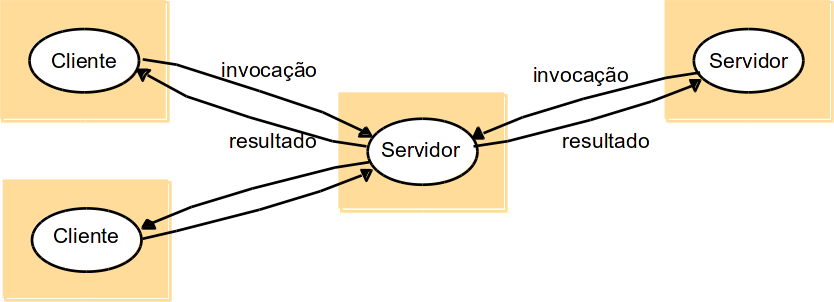
\includegraphics[scale=0.4]{cs2}%% Dimensões e localização
%     \fonte{Adaptado de \citeonline[p.~42]{Coulouris2013}}%% Fonte
%     \addcontentsline{loge}{figure}{\protect\numberline{\thefigure}Exemplo de figura criada a partir de um arquivo.}
% \end{figure}

% Utilizando o pacote \textit{subfig} é possível adicionar figuras lado a lado, como pode ser observado na \autoref{fig:exemplo3}.

% \begin{figure}[htb]
%     \caption{Telas de cadastro de Paciente: (a) Cadastro Paciente, (b) Cadastro Paciente 2} 
% 	\label{fig:exemplo3}
% 	\centering
% 	\subfloat[Cadastro Paciente]{
% 		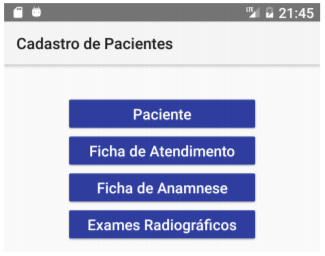
\includegraphics[scale=0.7]{cadastro-paciente}
% 	}\hspace{0.15cm} 
% 	\subfloat[Cadastro Paciente 2]{
% 		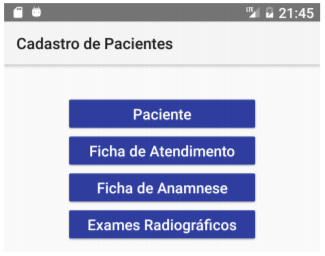
\includegraphics[scale=0.7]{cadastro-paciente}
% 	}	
% 	\fonte{}
%     %\addcontentsline{loge}{figure}{\protect\numberline{\thefigure}Telas de cadastro de Paciente: (a) Cadastro Paciente, (b) Cadastro Paciente 2.}
% \end{figure}

% Este modelo vem com o ambiente \texttt{quadro} e impressão de Lista de quadros configurados por padrão.  Este parágrafo apresenta como referenciar o quadro no texto, requisito obrigatório da \gls{abnt}. Primeira opção, utilizando \texttt{autoref}: Ver o \autoref{quad:exemplo1}. Segunda opção, utilizando  \texttt{ref}: Ver o Quadro \ref{quad:exemplo1}.

% \begin{tabframed}[htb]%% Ambiente tabframed
% %\captionsetup{width=0.5\textwidth}%% Largura da legenda
% \caption{Materiais utilizados no desenvolvimento do sistema}%% Legenda
% \label{quad:exemplo1}%% Rótulo
% \renewcommand{\arraystretch}{1.5}
% \begin{tabular}{|l|l|l|l|l}
% \cline{1-4}
% \textbf{Ferramenta/Tecnologia} & \textbf{Versão} & \textbf{Disponível em} & \textbf{Finalidade} \\ \cline{1-4}
%  Teste & 1.0  & https:/teste.org & Biblioteca de Teste & \\ \cline{1-4}  
%  Teste & 1.0  & https:/teste.org & Biblioteca de Teste & \\ \cline{1-4}
%  Teste & 1.0  & https:/teste.org & Biblioteca de Teste & \\ \cline{1-4}
%  Teste & 1.0  & https:/teste.org & Biblioteca de Teste & \\ \cline{1-4}
% \end{tabular}
% \fonte{}%% Fonte
% \addcontentsline{loge}{tabframed}{\protect\numberline{\thetabframed}Materiais utilizados no desenvolvimento do sistema.}
% \end{tabframed}


% Também é possível citar tabelas no texto. Primeira opção, utilizando \texttt{autoref}: Ver o \autoref{tab:exemplo1}. Segunda opção, utilizando  \texttt{ref}: Ver a Tabela \ref{tab:exemplo1}.

% \begin{table}[htb]
% % Luiz - O texto do caption da tabela/quadro deve ser do tamanho da tabela, então utilize a linha a seguir para conseguir esse efeito
% \captionsetup{width=0.83\textwidth}
% \centering
% \caption{\label{tab:exemplo1}Exemplo de tabela com uma legenda contendo um texto longo}
% \begin{tabular}{cccc}
% 	\hline
% 	\textbf{Pessoa} & \textbf{Idade} & \textbf{Peso} & \textbf{Altura} \\ \hline
% 	Marcos & 26    & 68   & 178    \\ 
% 	Ivone  & 22    & 57   & 162    \\ 
% 	...    & ...   & ...  & ...    \\ 
% 	Sueli  & 40    & 65   & 153    \\ \hline
% \end{tabular}
% \fonte{}
% \end{table}

% A \autoref{tab:exemplo2} também pode ser citada no texto.

% \begin{table}[htb]%% Ambiente table
% \caption{Segundo exemplo de tabela com uma legenda contendo um texto muito longo que pode ocupar mais de uma linha}%% Legenda
% \label{tab:exemplo2}%% Rótulo
% \begin{tabularx}{\textwidth}{@{\extracolsep{\fill}}llll}%% Ambiente tabularx
% \toprule
% $\bsym{L}$ & $\bsym{L^2}$ & $\bsym{L^3}$ & $\bsym{L^4}$ \\
% \SI{}{[m]} & \SI{}{[m^2]} & \SI{}{[m^3]} & \SI{}{[m^4]} \\ \midrule
% 1          & 1            & 1            & 1            \\
% 2          & 4            & 8            & 16           \\
% 3          & 9            & 27           & 81           \\
% 4          & 16           & 64           & 256          \\
% 5          & 25           & 125          & 625          \\ \bottomrule
% \end{tabularx}
% \fonte{}%% Fonte
% \end{table}

% A \autoref{tab:exemplo3} é um exemplo de tabela que ocupa mais de uma página e que foi construída pelo \gls{latex}\index{LaTeX@\latex} utilizando o pacote \texttt{longtable}.

% \begin{longtable}{@{\extracolsep{\fill}}lll}%% Ambiente longtable
% \caption{Possíveis tríplices para grade altamente variável\label{tab:exemplo3}} \\%% Legenda e rótulo
% \toprule
% \textbf{Tempo (s)} & \textbf{Tríplice escolhida} & \textbf{Outras possíveis tríplices} \\
% \midrule
% \endfirsthead%% Encerra cabeçalho da primeira página
% \caption[]{Possíveis tríplices para grade altamente variável} \\%% Legenda
% \multicolumn{3}{r}{\textbf{(continuação)}} \\
% \toprule
% \textbf{Tempo (s)} & \textbf{Tríplice escolhida} & \textbf{Outras possíveis tríplices} \\
% \midrule
% \endhead%% Encerra cabeçalho das demais páginas
% \midrule
% \multicolumn{3}{r}{\textbf{(continua)}} \\
% \endfoot%% Encerra rodapé das demais páginas
% \bottomrule
% \\[-0.5\linha]
% \caption*{\nomefonte: Adaptado de \citeonline[p.~42]{Smallen2014}} \\
% \endlastfoot%% Encerra rodapé da última página
% 0      & (1, 11, 13725) & (1, 12, 10980), (1, 13, 8235), (2, 2, 0), (3, 1, 0) \\
% 2745   & (1, 12, 10980) & (1, 13, 8235), (2, 2, 0), (2, 3, 0), (3, 1, 0)      \\
% 5490   & (1, 12, 13725) & (2, 2, 2745), (2, 3, 0), (3, 1, 0)                  \\
% 8235   & (1, 12, 16470) & (1, 13, 13725), (2, 2, 2745), (2, 3, 0), (3, 1, 0)  \\
% 10980  & (1, 12, 16470) & (1, 13, 13725), (2, 2, 2745), (2, 3, 0), (3, 1, 0)  \\
% 13725  & (1, 12, 16470) & (1, 13, 13725), (2, 2, 2745), (2, 3, 0), (3, 1, 0)  \\
% 16470  & (1, 13, 16470) & (2, 2, 2745), (2, 3, 0), (3, 1, 0)                  \\
% 19215  & (1, 12, 16470) & (1, 13, 13725), (2, 2, 2745), (2, 3, 0), (3, 1, 0)  \\
% 21960  & (1, 12, 16470) & (1, 13, 13725), (2, 2, 2745), (2, 3, 0), (3, 1, 0)  \\
% 24705  & (1, 12, 16470) & (1, 13, 13725), (2, 2, 2745), (2, 3, 0), (3, 1, 0)  \\
% 27450  & (1, 12, 16470) & (1, 13, 13725), (2, 2, 2745), (2, 3, 0), (3, 1, 0)  \\
% 30195  & (2, 2, 2745)   & (2, 3, 0), (3, 1, 0)                                \\
% 32940  & (1, 13, 16470) & (2, 2, 2745), (2, 3, 0), (3, 1, 0)                  \\
% 35685  & (1, 13, 13725) & (2, 2, 2745), (2, 3, 0), (3, 1, 0)                  \\
% 38430  & (1, 13, 10980) & (2, 2, 2745), (2, 3, 0), (3, 1, 0)                  \\
% 41175  & (1, 12, 13725) & (1, 13, 10980), (2, 2, 2745), (2, 3, 0), (3, 1, 0)  \\
% 43920  & (1, 13, 10980) & (2, 2, 2745), (2, 3, 0), (3, 1, 0)                  \\
% 46665  & (2, 2, 2745)   & (2, 3, 0), (3, 1, 0)                                \\
% 49410  & (2, 2, 2745)   & (2, 3, 0), (3, 1, 0)                                \\
% 52155  & (1, 12, 16470) & (1, 13, 13725), (2, 2, 2745), (2, 3, 0), (3, 1, 0)  \\
% 54900  & (1, 13, 13725) & (2, 2, 2745), (2, 3, 0), (3, 1, 0)                  \\
% 57645  & (1, 13, 13725) & (2, 2, 2745), (2, 3, 0), (3, 1, 0)                  \\
% 60390  & (1, 12, 13725) & (2, 2, 2745), (2, 3, 0), (3, 1, 0)                  \\
% 63135  & (1, 13, 16470) & (2, 2, 2745), (2, 3, 0), (3, 1, 0)                  \\
% 65880  & (1, 13, 16470) & (2, 2, 2745), (2, 3, 0), (3, 1, 0)                  \\
% 68625  & (2, 2, 2745)   & (2, 3, 0), (3, 1, 0)                                \\
% 71370  & (1, 13, 13725) & (2, 2, 2745), (2, 3, 0), (3, 1, 0)                  \\
% 74115  & (1, 12, 13725) & (2, 2, 2745), (2, 3, 0), (3, 1, 0)                  \\
% 76860  & (1, 13, 13725) & (2, 2, 2745), (2, 3, 0), (3, 1, 0)                  \\
% 79605  & (1, 13, 13725) & (2, 2, 2745), (2, 3, 0), (3, 1, 0)                  \\
% 82350  & (1, 12, 13725) & (2, 2, 2745), (2, 3, 0), (3, 1, 0)                  \\
% 85095  & (1, 12, 13725) & (1, 13, 10980), (2, 2, 2745), (2, 3, 0), (3, 1, 0)  \\
% 87840  & (1, 13, 16470) & (2, 2, 2745), (2, 3, 0), (3, 1, 0)                  \\
% 90585  & (1, 13, 16470) & (2, 2, 2745), (2, 3, 0), (3, 1, 0)                  \\
% 93330  & (1, 13, 13725) & (2, 2, 2745), (2, 3, 0), (3, 1, 0)                  \\
% 96075  & (1, 13, 16470) & (2, 2, 2745), (2, 3, 0), (3, 1, 0)                  \\
% 98820  & (1, 13, 16470) & (2, 2, 2745), (2, 3, 0), (3, 1, 0)                  \\
% 101565 & (1, 13, 13725) & (2, 2, 2745), (2, 3, 0), (3, 1, 0)                  \\
% 104310 & (1, 13, 16470) & (2, 2, 2745), (2, 3, 0), (3, 1, 0)                  \\
% 107055 & (1, 13, 13725) & (2, 2, 2745), (2, 3, 0), (3, 1, 0)                  \\
% 109800 & (1, 13, 13725) & (2, 2, 2745), (2, 3, 0), (3, 1, 0)                  \\
% 112545 & (1, 12, 16470) & (1, 13, 13725), (2, 2, 2745), (2, 3, 0), (3, 1, 0)  \\
% 115290 & (1, 13, 16470) & (2, 2, 2745), (2, 3, 0), (3, 1, 0)                  \\
% 118035 & (1, 13, 13725) & (2, 2, 2745), (2, 3, 0), (3, 1, 0)                  \\
% 120780 & (1, 13, 16470) & (2, 2, 2745), (2, 3, 0), (3, 1, 0)                  \\
% 123525 & (1, 13, 13725) & (2, 2, 2745), (2, 3, 0), (3, 1, 0)                  \\
% 126270 & (1, 12, 16470) & (1, 13, 13725), (2, 2, 2745), (2, 3, 0), (3, 1, 0)  \\
% 129015 & (2, 2, 2745)   & (2, 3, 0), (3, 1, 0)                                \\
% 131760 & (2, 2, 2745)   & (2, 3, 0), (3, 1, 0)                                \\
% 134505 & (1, 13, 16470) & (2, 2, 2745), (2, 3, 0), (3, 1, 0)                  \\
% 137250 & (1, 13, 13725) & (2, 2, 2745), (2, 3, 0), (3, 1, 0)                  \\
% 139995 & (2, 2, 2745)   & (2, 3, 0), (3, 1, 0)                                \\
% 142740 & (2, 2, 2745)   & (2, 3, 0), (3, 1, 0)                                \\
% 145485 & (1, 12, 16470) & (1, 13, 13725), (2, 2, 2745), (2, 3, 0), (3, 1, 0)  \\
% 148230 & (2, 2, 2745)   & (2, 3, 0), (3, 1, 0)                                \\
% 150975 & (1, 13, 16470) & (2, 2, 2745), (2, 3, 0), (3, 1, 0)                  \\
% 153720 & (1, 12, 13725) & (2, 2, 2745), (2, 3, 0), (3, 1, 0)                  \\
% 156465 & (1, 13, 13725) & (2, 2, 2745), (2, 3, 0), (3, 1, 0)                  \\
% 159210 & (1, 13, 13725) & (2, 2, 2745), (2, 3, 0), (3, 1, 0)                  \\
% 161955 & (1, 13, 16470) & (2, 2, 2745), (2, 3, 0), (3, 1, 0)                  \\
% 164700 & (1, 13, 13725) & (2, 2, 2745), (2, 3, 0), (3, 1, 0)                  \\
% \end{longtable}


% \subsection{Códigos fonte e algoritmos}\label{subsec:algoritimos}

% Os algoritmos podem ser utilizados para explicar uma determinada rotina desenvolvida. Conforme pode ser observado no \autoref{alg:exemplo1}.

% \begin{algorithm}[htb]%% Ambiente algorithm
% \caption{Algoritmo de exemplo}%% Legenda
% \label{alg:exemplo1}%% Rótulo
% \hrule
% \begin{algorithmic}[1]%% Ambiente algorithmic
% \ENSURE $A, B$
% \STATE $C = A + B$
% \IF{$C < 10$}
% \STATE $C = 2 \ C$
% \ELSE
% \STATE $C = 0,5 \ C$
% \ENDIF
% \PRINT $A, B, C$
% \end{algorithmic}
% \hrule
% \fonte{}%% Fonte
% \end{algorithm}

% \lipsum[1]

% \lipsum[1]

% Na \autoref{code:exemplo1} pode ser visualizado um exemplo de código fonte.

% \begin{sourcecode}[htb]
% \caption{\label{code:exemplo1}Exemplo de código}
% \begin{lstlisting}[frame=single, language=Java]
% @Entity
% public class Foo {
 
%     @Id
%     @GeneratedValue(strategy = GenerationType.IDENTITY)
%     private Long id;
 
%     private String name;
%     // constructor, getters and setters
% }
% \end{lstlisting}
% \fonte{}
% \end{sourcecode}

